\section{Ecossistema de software}

Ecossistema de software é definido, segundo \citeonline{manikas2013software},
como a interação entre diversos atores numa plataforma tecnológica comum,
resultando em novas soluções de software ou novos serviços. Atores do
ecossistema, motivados por um conjunto de interesses, conectam-se entre si e ao
próprio sistema numa relação simbiótica, fazendo a plataforma tecnológica
evoluir enquanto permite o envolvimento e contribuição de novos e diferentes
atores \cite{manikas2013software}.

Nesta relação, os atores são beneficiados de formas diferentes a depender da
natureza do ecossistema. Num ambiente comercial, por exemplo, os atores são
beneficiados diretamente através de receita financeira (salário, prêmios, etc),
enquanto num sistema não-comercial os atores estão motivados por questões
não-monetárias, como fama, reconhecimento, ideologia, etc
\cite{manikas2013software}.

De modo geral, em ecossistemas de software, os benefícios recebidos pelos
atores e proporcionados pelo ecossistema, aumentam com o passar do tempo por
meio de uma relação de benefício mútuo.  Este modelo geral de funcionamento, no
entanto, pode variar a depender do contexto em que se insere o ecossistema,
especialmente no relacionamento entre os atores que pode variar entre
mutualismo, parasitismo, antagonismo e competição
\cite{manikas2013software}.

\section{Ecossistema de software acadêmico}

O ecossistema de software acadêmico possui a particularidade de se relacionar
com o sistema econômico de reputação científica, especialmente com o seu modelo
de publicações, influenciando e sendo influenciado diretamente pelo impacto de
suas publicações \cite{howison2015understanding}.

Neste cenário, interessado em compreender as relações neste ecossistema,
\citeonline{howison2015understanding} criou um framework para pensar e refletir
sobre o processo de produção de software no meio científico, e identificou quatro
papéis básicos assumidos pelos atores envolvidos no ecossistema de software acadêmico: 
(1) cientistas usuários finais, (2) produtores e distribuidores de software, (3)
administradores de infraestrutura e (4) pesquisadores preocupados com o
funcionamento do ecossistema como um todo.

\subsection{Cientistas usuários finais}

Cientistas ocupam papel chave no ecossistema de software acadêmico.  Em seus
processos de investigação e experimentação, fazem uso crescente de software
para coleta, gerenciamento, transformação, análise, modelagem e visualização de
dados. Além da preocupação com qualidade e usabilidade, estes cientistas estão
também preocupados com a disponibilidade e com a capacidade do software em
continuar sendo útil \cite{howison2015understanding}.

Estão interessados também em saber o que outros
cientistas estão usando em suas pesquisas. A alta adoção de um software, além
de ser um bom indicador de qualidade, mantém os cientistas mais livres e com
maior foco em suas próprias pesquisas, uma vez que podem encontrar ajuda entre
os seus pares para resolver questões sobre o uso do software
\cite{howison2015understanding}.

\subsection{Produtor e distribuidor de software acadêmico}

O papel de produtor e distribuidor de software costuma ser desempenhado por
equipes colaborando entre sí, geralmente compostas por cientistas da computação
e cientistas do domínio onde a pesquisa se insere.
Geralmente, o cientista da computação é o responsável por implementar os
algoritmos, métodos ou resultados gerados pelo estudo
\cite{howison2015understanding}.

Um desafio comum enfrentado neste papel é conseguir abstrair os problemas e
implementar soluções abrangentes em software.
Muitas vezes, o software criado fica confinado em seu laboratório ou grupo, mas
eventualmente é compartilhado e amplamente adotado, tornando o cientista autor
do software e da pesquisa parte do seu ecossistema \cite{howison2015understanding}.

Entre as inúmeras preocupações do produtor e distribuidor de software, podemos
destacar a preocupação acerca de como o software contribui para as
investigações científicas que outros pesquisadores estão realizando.
Alguns projetos são gerenciados no estilo de código aberto, e têm atraído com
sucesso contribuições de muitos cientistas, incluindo contribuidores que
fazem pequenas, porém substanciais contribuições
\cite{howison2015understanding}.

\subsection{Provedor de infraestrutura}

O provedor de infraestrutura é aquele que provê cojuntos de software aos
cientistas usuários finais. Este conjunto pode estar disponível em forma de
download para que seja utilizado em computadores pessoais ou pode estar
disponível em forma de serviços, como por exemplo, ciberinfraestrutura
de software \cite{council2007cyberinfrastructure, stewart2010cyberinfrastructure}.

Do ponto de vista do ecossistema, os dois tipos de distribuição implicam nas
mesmas preocupações e questões: quem usa o software, qual versão é utilizada, 
qual a frequencia de atualização, entre outras \cite{howison2015understanding}.

\subsection{Pesquisador}

Este último papel, chamado de pesquisador num sentido amplo, refere-se a
qualquer pessoa preocupada com o funcionamento do ecossistema e com a sua
contribuição para a Ciência. O papel de pesquisador costuma ser desempenhado
por agências de fomento ou por cientistas preocupados com o seu trabalho
individual e com o impacto em seu campo de pesquisa
\cite{howison2015understanding}.

As preocupações incluem questões sobre a operação do ecossistema
como um sistema que consome recursos (tempo, dinheiro e atenção) e afeta a
conduta da ciência, tanto no geral como em campos específicos, 
e sobre a compreensão do comportamento desse sistema e de 
como pode ser influenciado \cite{howison2015understanding}.

\section{Modelo de desenvolvimento de software acadêmico}

Cada ator desempenha um papel importante na estabilidade e sustentabilidade do
ecossistema \cite{dhungana2010software}. Assim como nos ecossistemas naturais,
o ecossistema de software necessita de fornecimento constante de energia, seja
na forma de novos desenvolvimentos ou na forma de ações de manutenção
\cite{dhungana2010software}.

Os atores participam dentro de seus próprios interesses, mas sempre causando
impacto no sistema como um todo \cite{manikas2013software}.
Cientistas usuários finais usam software acadêmico (direta ou indiretamente)
para fazer Ciência, resultando em impacto científico. Tal impacto científico
justifica novos investimentos, fazendo o ecossistema crescer
\cite{howison2015understanding}.

\begin{figure}[h]
  \center
  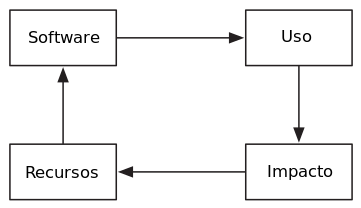
\includegraphics[scale=0.5]{imagens/process-model-scientific-software-dia.png}
  \caption{Um modelo de processo de software na Ciência~\cite{howison2015understanding}}
  \label{process-model-scientific-software}
\end{figure}

A Figura \ref{process-model-scientific-software} apresenta um modelo de
desenvolvimento de software acadêmico, explicitando as relações entre os
elementos \textit{software}, \textit{recursos}, \textit{uso} e
\textit{impacto}, detalhados a seguir.

\subsection{Software acadêmico}

Software acadêmico ({\it academic software}) é todo software usado para
coletar, processar ou analisar resultados de pesquisas com intenção de
publicação na literatura acadêmica (periódicos, revistas, conferências,
monografias, livros ou teses), incluindo desde protótipos escritos pelos
próprios cientistas, a produtos completos desenvolvidos profissionalmente
\cite{allen2017engineering}.

Podem ser projetos de software desenvolvidos num modelo de {\bf Software como
serviço de suporte} ({\it Software as Supporting Service}), sobrevivendo
totalmente à parte do sistema de reputação acadêmica, ou no modelo de {\bf
Software para crédito acadêmico} ({\it Software for academic credit}), estando
seu desenvolvimento intrinsecamente associado ao sistema de reputação acadêmica
\cite{howison2011scientific}.

No segundo caso, Software para crédito acadêmico, a relação com o sistema de
reputação acadêmica pode ainda variar entre motivações distintas resultando em
(1) Software Incidental ({\it Incidental software})
feito puramente para apoiar e facilitar pesquisas,
(2) Prática de software paralela ({\it A parallel software practice})
feito com objetivo de ser utilizado por outros pesquisadores, ou
(3) Um subcampo de software ({\it A Software Subfield}),
onde o próprio software é considerado uma contribuição primária para a Ciência
\cite{howison2011scientific}.

\subsection{Recursos}

Os recursos investidos na produção de software acadêmico vêm de diversas
fontes, incluindo ganhos monetários diretos, recursos alocados em projetos, e
colaboração entre laboratórios de pesquisa \cite{howison2015understanding}.
Grande parte dos recursos vem do ``tempo livre'' dos pesquisadores em busca de
soluções para suas pesquisas e perpassa por financiamentos diversos obtidos na
carreira individual do cientista, prêmios recebidos, etc
\cite{howison2015understanding}.

Independente da origem dos recursos, grande parte do desenvolvimento de
software acadêmico é realizado pelos próprios cientistas \cite{hettrick2014uk,
momcheva2015software}.
Esta tendência tem sido interpretada como um reflexo do conhecimento sobre o
domínio da pesquisa muitas vezes necessário ao ator desenvolvedor do software
\cite{segal2008developing}.

Nas pesquisas em Engenharia de Software, este conhecimento teórico sobre o
domínio da pesquisa se confunde, muitas vezes, com a própria prática de
desenvolvimento de software, especialmente no domínio de análise estática, uma
área intimamente ligada a pesquisas sobre a construção de software,
como linguagens e compiladores, por exemplo.

\subsection{Uso}

Metade dos pesquisadores de todas as áreas da Ciência fazem uso intenso de
software acadêmico, desde grupos trabalhando exclusivamente com problemas
computacionais até grupos em laboratórios tradicionais ou em campo
\cite{wilson2014best}.

Este uso é mencionado na literatura academica por meio de citação formal ou informal
\cite{smith2016software} e está estreitamente relacionado ao sistema
econômico de reputação científica, uma vez que
menções causam
impacto científico direto tanto na publicação quanto no ecossistema de software
acadêmico \cite{katz2014transitive}.

Este impacto direto geralmente justifica o investimentos de novos recursos no
ecossistema, seja para fins de planejamento, por exemplo, uma retrospectiva para avaliar
investimentos já realizados ou para fins de promoção e evolução do software acadêmico
\cite{howison2015understanding}.

\subsection{Impacto científico}

Ao longo da história, a citação formal tem sido utilizada para garantir
autenticidade e autoridade, ao invés de crédito e reconhecimento
\cite{katz2014transitive}.
Na história ocidental, a citação surge no final do século XVI e, no início do
século XVIII surgem o sistema legal por trás do sistema de citações e a lei de
``copyright'' para garantir os direitos dos autores \cite{katz2014transitive}.

Apesar desse uso histórico para fins de autenticidade e autoridade, o sistema de
citações e as informaçãos de autoria das publicações tem sido
utilizado para avaliações importantes dentro do corpo científico
\cite{katz2014transitive}.
Por exemplo, para realizar ``backward citing'' o sistema tem sido utilizado para se certificar quem de
fato contribuiiu para um certo avanço ou descoberta, e ``forward citing'' tem
sido usada em casos onde se quer entender como uma idéia foi usada após o seu
surgimento ou publicação \cite{katz2014transitive}.

Conhecimento novo é claramente construído a partir do conhecimento passado e o
sistema de citações formais tem promovido avanços significativos
\cite{katz2014transitive}.
No entanto, esse conceito não tem funcionado tão bem para produtos digitais
como o software, que muitas vezes depende de outro software, fragmentos de
código, e algoritmos \cite{katz2014transitive}.

Este debate ocorre há bastante tempo entre as diversas áreas da bibliometria,
cienciometria, altmetria e áreas similares \cite{gouveia2013altmetria}.
O fator de impacto, por exemplo, proposto na década de 90
\cite{reuters2017history}, apesar de contribuir para a Ciência, por
vezes é utilizado da forma errada e mostra as deficiências de lidar bem com
produtos digitais gerados durante pesquisas \cite{katz2014transitive}.
